% ARTICLE 2 ----
% This is just here so I know exactly what I'm looking at in Rstudio when messing with stuff.
% Options for packages loaded elsewhere
\PassOptionsToPackage{unicode}{hyperref}
\PassOptionsToPackage{hyphens}{url}
%
\documentclass[
  11pt,
]{article}
\usepackage{lmodern}
\usepackage{amssymb,amsmath}
\usepackage{ifxetex,ifluatex}
\ifnum 0\ifxetex 1\fi\ifluatex 1\fi=0 % if pdftex
  \usepackage[T1]{fontenc}
  \usepackage[utf8]{inputenc}
  \usepackage{textcomp} % provide euro and other symbols
\else % if luatex or xetex
  \usepackage{unicode-math}
  \defaultfontfeatures{Scale=MatchLowercase}
  \defaultfontfeatures[\rmfamily]{Ligatures=TeX,Scale=1}
  \setmainfont[]{cochineal}
\fi
% Use upquote if available, for straight quotes in verbatim environments
\IfFileExists{upquote.sty}{\usepackage{upquote}}{}
\IfFileExists{microtype.sty}{% use microtype if available
  \usepackage[]{microtype}
  \UseMicrotypeSet[protrusion]{basicmath} % disable protrusion for tt fonts
}{}
\makeatletter
\@ifundefined{KOMAClassName}{% if non-KOMA class
  \IfFileExists{parskip.sty}{%
    \usepackage{parskip}
  }{% else
    \setlength{\parindent}{0pt}
    \setlength{\parskip}{6pt plus 2pt minus 1pt}
    }
}{% if KOMA class
  \KOMAoptions{parskip=half}}
\makeatother
\usepackage{xcolor}
\IfFileExists{xurl.sty}{\usepackage{xurl}}{} % add URL line breaks if available
\urlstyle{same} % disable monospaced font for URLs
\usepackage[margin=1in]{geometry}
\usepackage{color}
\usepackage{fancyvrb}
\newcommand{\VerbBar}{|}
\newcommand{\VERB}{\Verb[commandchars=\\\{\}]}
\DefineVerbatimEnvironment{Highlighting}{Verbatim}{commandchars=\\\{\}}
% Add ',fontsize=\small' for more characters per line
\usepackage{framed}
\definecolor{shadecolor}{RGB}{248,248,248}
\newenvironment{Shaded}{\begin{snugshade}}{\end{snugshade}}
\newcommand{\AlertTok}[1]{\textcolor[rgb]{0.94,0.16,0.16}{#1}}
\newcommand{\AnnotationTok}[1]{\textcolor[rgb]{0.56,0.35,0.01}{\textbf{\textit{#1}}}}
\newcommand{\AttributeTok}[1]{\textcolor[rgb]{0.77,0.63,0.00}{#1}}
\newcommand{\BaseNTok}[1]{\textcolor[rgb]{0.00,0.00,0.81}{#1}}
\newcommand{\BuiltInTok}[1]{#1}
\newcommand{\CharTok}[1]{\textcolor[rgb]{0.31,0.60,0.02}{#1}}
\newcommand{\CommentTok}[1]{\textcolor[rgb]{0.56,0.35,0.01}{\textit{#1}}}
\newcommand{\CommentVarTok}[1]{\textcolor[rgb]{0.56,0.35,0.01}{\textbf{\textit{#1}}}}
\newcommand{\ConstantTok}[1]{\textcolor[rgb]{0.00,0.00,0.00}{#1}}
\newcommand{\ControlFlowTok}[1]{\textcolor[rgb]{0.13,0.29,0.53}{\textbf{#1}}}
\newcommand{\DataTypeTok}[1]{\textcolor[rgb]{0.13,0.29,0.53}{#1}}
\newcommand{\DecValTok}[1]{\textcolor[rgb]{0.00,0.00,0.81}{#1}}
\newcommand{\DocumentationTok}[1]{\textcolor[rgb]{0.56,0.35,0.01}{\textbf{\textit{#1}}}}
\newcommand{\ErrorTok}[1]{\textcolor[rgb]{0.64,0.00,0.00}{\textbf{#1}}}
\newcommand{\ExtensionTok}[1]{#1}
\newcommand{\FloatTok}[1]{\textcolor[rgb]{0.00,0.00,0.81}{#1}}
\newcommand{\FunctionTok}[1]{\textcolor[rgb]{0.00,0.00,0.00}{#1}}
\newcommand{\ImportTok}[1]{#1}
\newcommand{\InformationTok}[1]{\textcolor[rgb]{0.56,0.35,0.01}{\textbf{\textit{#1}}}}
\newcommand{\KeywordTok}[1]{\textcolor[rgb]{0.13,0.29,0.53}{\textbf{#1}}}
\newcommand{\NormalTok}[1]{#1}
\newcommand{\OperatorTok}[1]{\textcolor[rgb]{0.81,0.36,0.00}{\textbf{#1}}}
\newcommand{\OtherTok}[1]{\textcolor[rgb]{0.56,0.35,0.01}{#1}}
\newcommand{\PreprocessorTok}[1]{\textcolor[rgb]{0.56,0.35,0.01}{\textit{#1}}}
\newcommand{\RegionMarkerTok}[1]{#1}
\newcommand{\SpecialCharTok}[1]{\textcolor[rgb]{0.00,0.00,0.00}{#1}}
\newcommand{\SpecialStringTok}[1]{\textcolor[rgb]{0.31,0.60,0.02}{#1}}
\newcommand{\StringTok}[1]{\textcolor[rgb]{0.31,0.60,0.02}{#1}}
\newcommand{\VariableTok}[1]{\textcolor[rgb]{0.00,0.00,0.00}{#1}}
\newcommand{\VerbatimStringTok}[1]{\textcolor[rgb]{0.31,0.60,0.02}{#1}}
\newcommand{\WarningTok}[1]{\textcolor[rgb]{0.56,0.35,0.01}{\textbf{\textit{#1}}}}
\usepackage{graphicx}
\makeatletter
\def\maxwidth{\ifdim\Gin@nat@width>\linewidth\linewidth\else\Gin@nat@width\fi}
\def\maxheight{\ifdim\Gin@nat@height>\textheight\textheight\else\Gin@nat@height\fi}
\makeatother
% Scale images if necessary, so that they will not overflow the page
% margins by default, and it is still possible to overwrite the defaults
% using explicit options in \includegraphics[width, height, ...]{}
\setkeys{Gin}{width=\maxwidth,height=\maxheight,keepaspectratio}
% Set default figure placement to htbp
\makeatletter
\def\fps@figure{htbp}
\makeatother
\setlength{\emergencystretch}{3em} % prevent overfull lines
\providecommand{\tightlist}{%
  \setlength{\itemsep}{0pt}\setlength{\parskip}{0pt}}
\setcounter{secnumdepth}{-\maxdimen} % remove section numbering

\ifluatex
  \usepackage{selnolig}  % disable illegal ligatures
\fi
\usepackage[]{natbib}
\bibliographystyle{apsr}


\title{Another Pandoc Markdown Article Starter and
Template\thanks{Replication files are available on the author's Github
account (\url{http://github.com/svmiller/svm-r-markdown-templates}).
\textbf{Current version}: May 02, 2021; \textbf{Corresponding author}:
\href{mailto:steven.v.miller@gmail.com}{\nolinkurl{steven.v.miller@gmail.com}}.}}
\author{true \and true \and true}
\date{May 02, 2021}

% Jesus, okay, everything above this comment is default Pandoc LaTeX template. -----
% ----------------------------------------------------------------------------------
% I think I had assumed beamer and LaTex were somehow different templates.


\usepackage{kantlipsum}

\usepackage{abstract}
\renewcommand{\abstractname}{}    % clear the title
\renewcommand{\absnamepos}{empty} % originally center

\renewenvironment{abstract}
 {{%
    \setlength{\leftmargin}{0mm}
    \setlength{\rightmargin}{\leftmargin}%
  }%
  \relax}
 {\endlist}

\makeatletter
\def\@maketitle{%
  \newpage
%  \null
%  \vskip 2em%
%  \begin{center}%
  \let \footnote \thanks
      {\fontsize{18}{20}\selectfont\raggedright  \setlength{\parindent}{0pt} \@title \par}
    }
%\fi
\makeatother


\title{Another Pandoc Markdown Article Starter and
Template\thanks{Replication files are available on the author's Github
account (\url{http://github.com/svmiller/svm-r-markdown-templates}).
\textbf{Current version}: May 02, 2021; \textbf{Corresponding author}:
\href{mailto:steven.v.miller@gmail.com}{\nolinkurl{steven.v.miller@gmail.com}}.}  }

\date{}

\usepackage{titlesec}

% 
\titleformat*{\section}{\large\bfseries}
\titleformat*{\subsection}{\normalsize\itshape} % \small\uppercase
\titleformat*{\subsubsection}{\normalsize\itshape}
\titleformat*{\paragraph}{\normalsize\itshape}
\titleformat*{\subparagraph}{\normalsize\itshape}

% add some other packages ----------

% \usepackage{multicol}
% This should regulate where figures float
% See: https://tex.stackexchange.com/questions/2275/keeping-tables-figures-close-to-where-they-are-mentioned
\usepackage[section]{placeins}



\makeatletter
\@ifpackageloaded{hyperref}{}{%
\ifxetex
  \PassOptionsToPackage{hyphens}{url}\usepackage[setpagesize=false, % page size defined by xetex
              unicode=false, % unicode breaks when used with xetex
              xetex]{hyperref}
\else
  \PassOptionsToPackage{hyphens}{url}\usepackage[draft,unicode=true]{hyperref}
\fi
}

\@ifpackageloaded{color}{
    \PassOptionsToPackage{usenames,dvipsnames}{color}
}{%
    \usepackage[usenames,dvipsnames]{color}
}
\makeatother
\hypersetup{breaklinks=true,
            bookmarks=true,
            pdfauthor={Steven V. Miller (Clemson University) and A
Second Author Who Did Less Work (The Ohio State University) and A
Graduate Student (University of Alabama)},
             pdfkeywords = {pandoc, r markdown, knitr},
            pdftitle={Another Pandoc Markdown Article Starter and
Template},
            colorlinks=true,
            citecolor=blue,
            urlcolor=blue,
            linkcolor=magenta,
            pdfborder={0 0 0}}
\urlstyle{same}  % don't use monospace font for urls

% Add an option for endnotes. -----



% This will better treat References as a section when using natbib
% https://tex.stackexchange.com/questions/49962/bibliography-title-fontsize-problem-with-bibtex-and-the-natbib-package
\renewcommand\bibsection{%
   \section*{References}%
   \markboth{\MakeUppercase{\refname}}{\MakeUppercase{\refname}}%
  }%

% set default figure placement to htbp
\makeatletter
\def\fps@figure{htbp}
\makeatother



\usepackage{longtable}
\LTcapwidth=.95\textwidth
\linespread{1.05}
\usepackage{hyperref}

\newtheorem{hypothesis}{Hypothesis}


% trick for moving figures to back of document
% really wish we'd knock this shit off with moving tables/figures to back of document
% but, alas...


\begin{document}

% \textsf{\textbf{This is sans-serif bold text.}}
% \textbf{\textsf{This is bold sans-serif text.}}


% \maketitle

{% \usefont{T1}{pnc}{m}{n}
\setlength{\parindent}{0pt}
\thispagestyle{plain}
{%\fontsize{18}{20}\selectfont\raggedright
\maketitle  % title \par

}




{
   \vskip 13.5pt\relax \normalsize\fontsize{11}{12}
   \MakeUppercase{Steven V. Miller}, \small{Clemson
University}   \par \vskip -3.5pt \MakeUppercase{A Second Author Who Did
Less Work}, \small{The Ohio State
University}   \par \vskip -3.5pt \MakeUppercase{A Graduate
Student}, \small{University of Alabama}   

}

}








\begin{abstract}

%    \hbox{\vrule height .2pt width 39.14pc}

    \vskip 8.5pt % \small

\noindent \small{Lorem ipsum dolor sit amet, consectetur adipiscing
elit. Donec sit amet libero justo. Pellentesque eget nibh ex. Aliquam
tincidunt egestas lectus id ullamcorper. Proin tellus orci, posuere sed
cursus at, bibendum ac odio. Nam consequat non ante eget aliquam. Nulla
facilisis tincidunt elit. Nunc hendrerit pellentesque quam, eu imperdiet
ipsum porttitor ut. Interdum et malesuada fames ac ante ipsum primis in
faucibus. Suspendisse potenti. Duis vitae nibh mauris. Duis nec sem sit
amet ante dictum mattis. Suspendisse diam velit, maximus eget commodo
at, faucibus et nisi. Ut a pellentesque eros, sit amet suscipit eros.
Nunc tincidunt quis risus suscipit vestibulum. Quisque eu fringilla
massa.}


\vskip 8.5pt \noindent \emph{Keywords}: pandoc, r markdown, knitr \par

%    \hbox{\vrule height .2pt width 39.14pc}



\end{abstract}


\vskip -8.5pt


 % removetitleabstract


\setlength{\parindent}{16pt}
\setlength{\parskip}{0pt}

% We'll put doublespacing here
% Remember to cut it out later before bib
\hypertarget{introduction}{%
\section{Introduction}\label{introduction}}

\kant[1]

\hypertarget{a-subsection-in-the-introduction}{%
\subsection{A Subsection in the
Introduction}\label{a-subsection-in-the-introduction}}

\kant[2]

This is an R Markdown document. Markdown is a simple formatting syntax
for authoring HTML, PDF, and MS Word documents. For more details on
using R Markdown see \url{http://rmarkdown.rstudio.com}.

When you click the \textbf{Knit} button a document will be generated
that includes both content as well as the output of any embedded R code
chunks within the document. You can embed an R code chunk like this:

\begin{Shaded}
\begin{Highlighting}[]
\FunctionTok{summary}\NormalTok{(cars)}
\end{Highlighting}
\end{Shaded}

\begin{verbatim}
##      speed           dist       
##  Min.   : 4.0   Min.   :  2.00  
##  1st Qu.:12.0   1st Qu.: 26.00  
##  Median :15.0   Median : 36.00  
##  Mean   :15.4   Mean   : 42.98  
##  3rd Qu.:19.0   3rd Qu.: 56.00  
##  Max.   :25.0   Max.   :120.00
\end{verbatim}

\hypertarget{results}{%
\section{Results}\label{results}}

\kant[24]

\hypertarget{including-plots}{%
\subsection{Including Plots}\label{including-plots}}

You can also embed plots, for example:

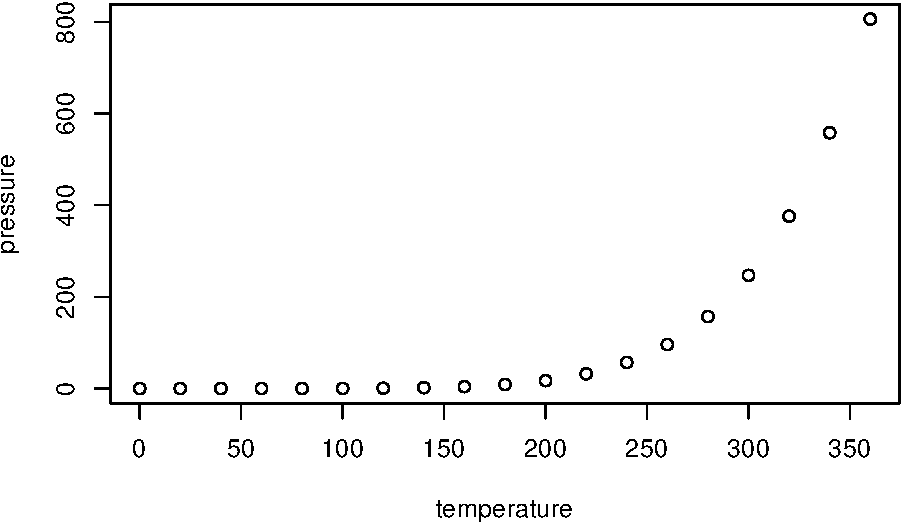
\includegraphics{demo_2_files/figure-latex/pressure-1.pdf}

Note that the \texttt{echo\ =\ FALSE} parameter was added to the code
chunk to prevent printing of the R code that generated the plot.

\kant[25]

\begin{Shaded}
\begin{Highlighting}[]
\FunctionTok{plot}\NormalTok{(mtcars)}
\end{Highlighting}
\end{Shaded}

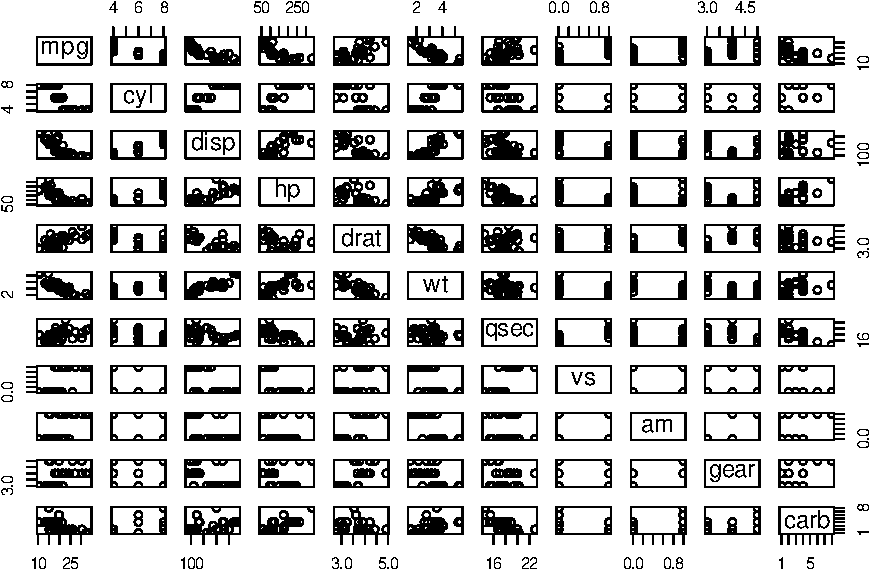
\includegraphics{demo_2_files/figure-latex/unnamed-chunk-1-1.pdf}

\end{document}
